\section{Analysis}
\label{sec:analysis}

\subsection{Experiment Setup}
\label{subsec:exp_setup}

In order to evaluate this software, the authors ran two series of tests: one that ran the application with 8 ranks per node and another that ran with 16 ranks per node.  Each series included tests of the daemon using 1, 2, and 4 background write threads.  Both series also tested the write performance just using standard \texttt{write()} calls in order to get some baseline data for comparison.

For the first test series, the application was configured for 8 ranks per node.  As mentioned in the introduction, `real' applications will often run on Titan using only 8 ranks per node because the AMD processor in the compute nodes only has 8 floating point units.  From the authors' perspective, this has the advantage of leaving 8 integer-only cores to run the daemon in multi-threaded mode.  For this test series, aprun was configured to pin the application ranks to the even numbered cores and the daemon was configured to pin its threads to odd numbered cores.  Furthermore, the daemon thread that processed the CCI messages was run in a mode where it continuously polled for new messages.  This  provided the lowest possible latency for message handling, but at the cost of effectively consuming one core. 

For the second test series, the application was configured for 16 ranks per node.  The daemon was again run with 1, 2, and 4 write threads.  For this series, the daemon thread that handled the CCI messages was run in a mode where it would block waiting on a message.  This added some latency to the message processing, but left that core free to perform useful work when there were no messages to process.  Also for this series, no core pinning was used on the daemon.\footnote{In practical terms, a user would probably not want to use multiple write threads on the daemon if his/her application was running 16 ranks/node since it would oversubscribe the cores.  The authors tested the daemon with 2 and 4 threads partially out of curiosity and also to keep the two test series as similar to each other as possible.}   

For both test series, the daemon was configured to write each rank's data to a separate file and the test measured the application's perceived write performance as the write size increased.  Note the word `perceived'.  What was actually measured was how long it took for each rank of the application to copy its data into GPU memory.   The GPU cards in each of Titan's compute nodes have 6GB of RAM, though in practice only a little over 5GB is actually available to the user.  This means that for the first test series, with 8 ranks per node, write sizes of up to 512 MB were small enough for all ranks' writes to fit into GPU memory.  For the second test series, using 16 ranks per node, write sizes up to 256MB would fit.  For both test series, once the write size exceeded the available GPU memory, the ranks would have to wait until the daemon was able to drain data out of GPU memory and into the filesystem page cache or over the network.


\subsection{Results}
\label{subsec:results}

\begin{figure}
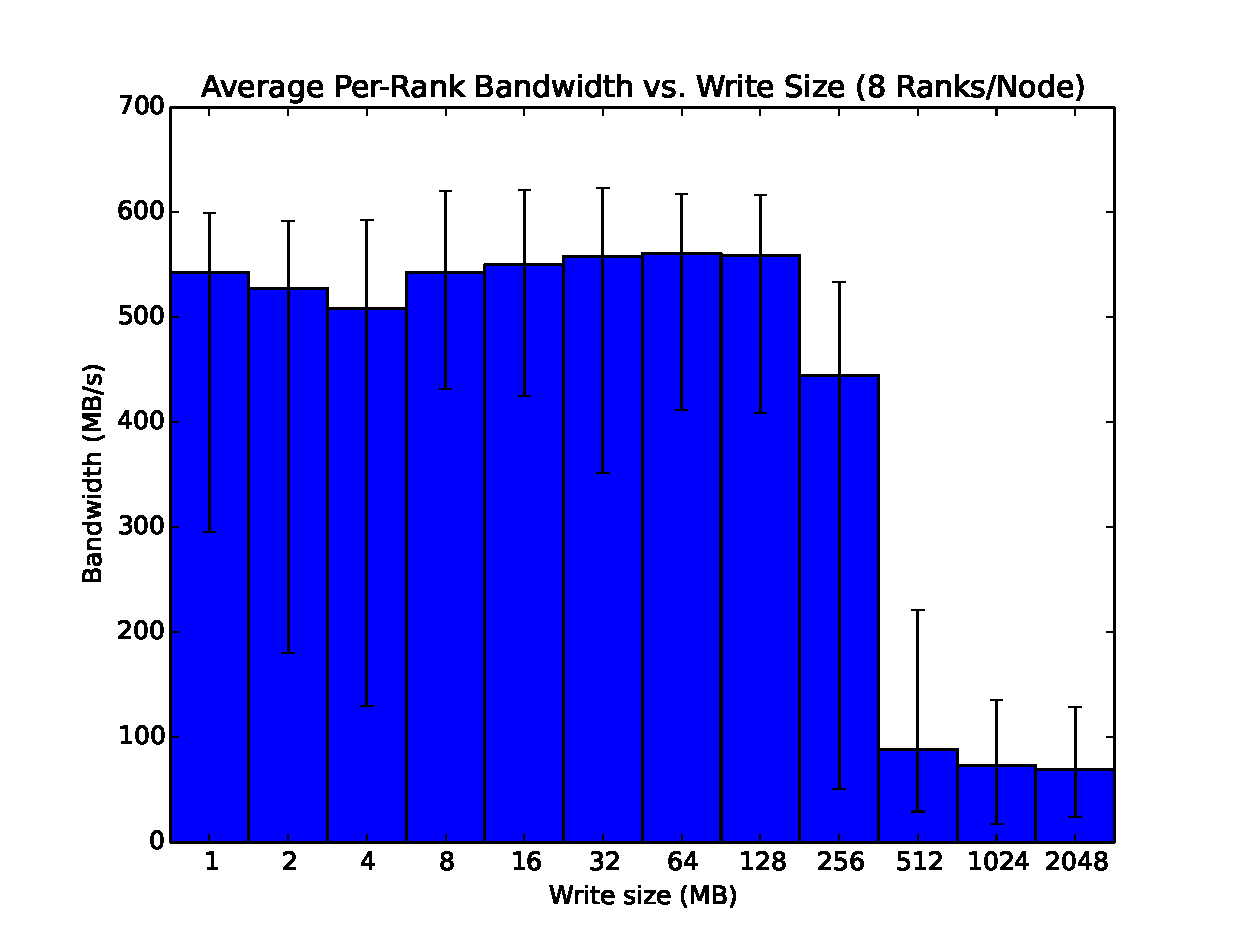
\includegraphics[width=\linewidth]{figures/figure_1.eps}
\caption{Average per-rank write bandwidth using standard \texttt{write()} calls.  8 ranks per node. No GPU memory cache.} 
\label{fig:results_base_8}
\end{figure}

Figure \ref{fig:results_base_8} shows the results of a baseline test.  The colored bars show the average throughput for 128 nodes and the error bars display the minimum and maximum values.  In this test, the application wrote to the filesystem with standard \texttt{write()} calls and the GPU memory was not used at all.\footnote{The daemon process was not even started for this test.}  The results provide some baseline numbers that can be used for comparison with the tests using GPU memory.

Note the sharp drop in performance between 256MB and 512MB.  On Titan, the Lustre client is configured to allow a maximum of 64MB per OST and to default to using 4 OSTs per file.  Given the number of OSTs available, it is statistically likely that no two output files in this test used the same OSTs.  In short, write sizes of 256MB or less were cached in system memory using the existing Lustre client cache and the performance of the 512MB, 1GB and 2GB sizes is dominated by the performance of the filesystem.  In order for this work to be useful, it must obviously improve on that.

\begin{figure}
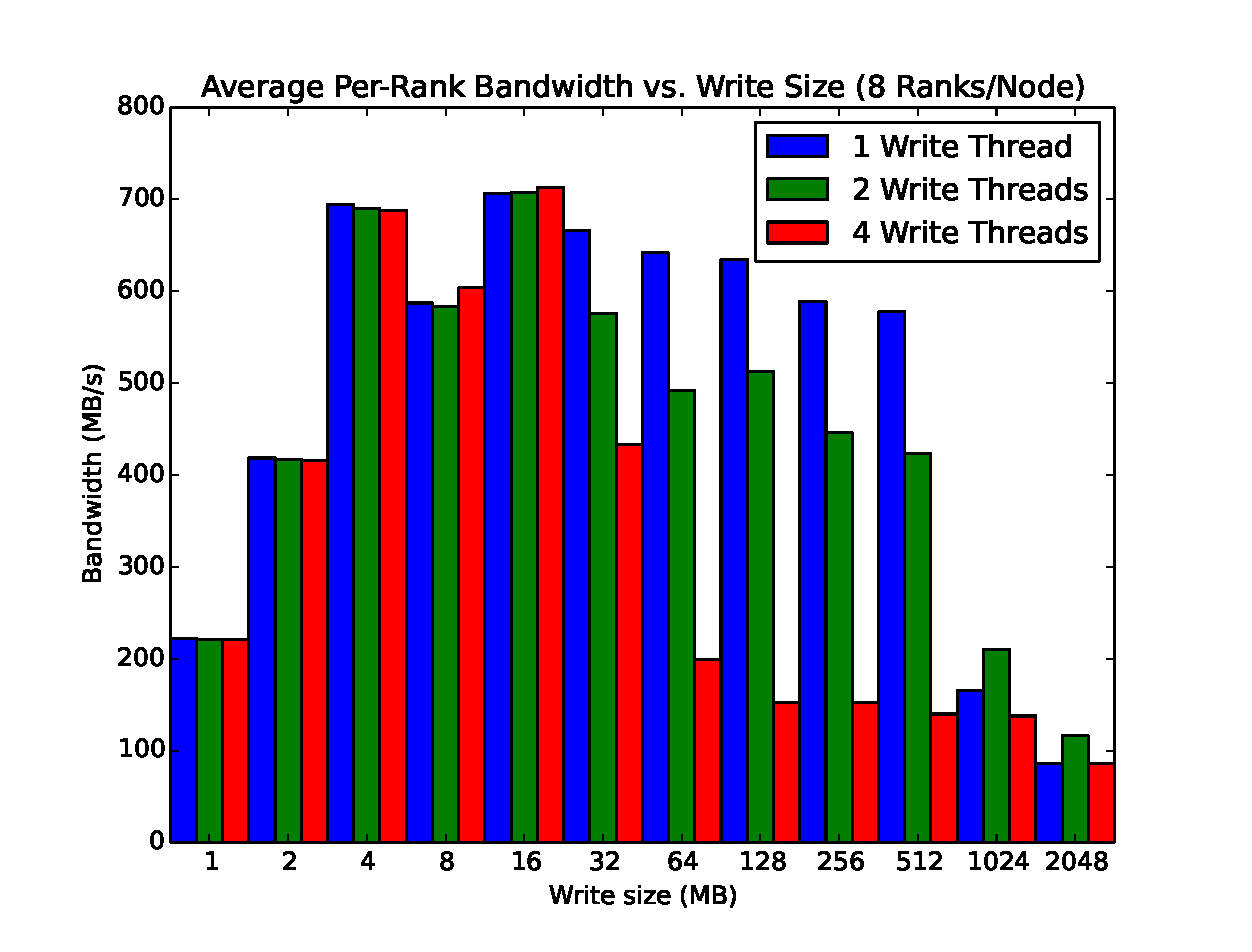
\includegraphics[width=\linewidth]{figures/figure_2.eps}
\caption{Average per-rank write bandwidth.  8 ranks per node.} 
\label{fig:results_8_nobars}
\end{figure}

Figure \ref{fig:results_8_nobars} shows the remaining results of the first test series.  As stated earlier, this series was run with 8 ranks per node and with 1, 2, and 4 write threads in the daemon. Each column is the mean of 64 nodes' perceived per-process throughput. The graph shows a number of interesting features.  The first and most obvious, is that multiple write threads decrease performance.  Exactly why this is so is unclear, but it appears that having multiple threads read from GPU memory interfered with the individual ranks' ability to copy data into GPU memory.  

Concentrating on the single thread performance, it is clear that the application benefits from using GPU memory out to the 512MB write size.  This makes sense since eight ranks each writing 512MB is a total of 4GB and that will fit into the available GPU memory.  Even at 1GB, the application sees somewhat improved performance because there is enough GPU memory to hold significant fraction of the data to be written.  It is not until the 2GB write size that the write performance is dominated by the filesystem's throughput.

Also obvious from the graph is the fact that small write sizes are not particularly efficient.  For write sizes less than 4MB, copying data to GPU memory is slower than writing to the Lustre cache.  This is not surprising given the results shown in Figure \ref{fig:transfer_bw}.


%\begin{figure}
%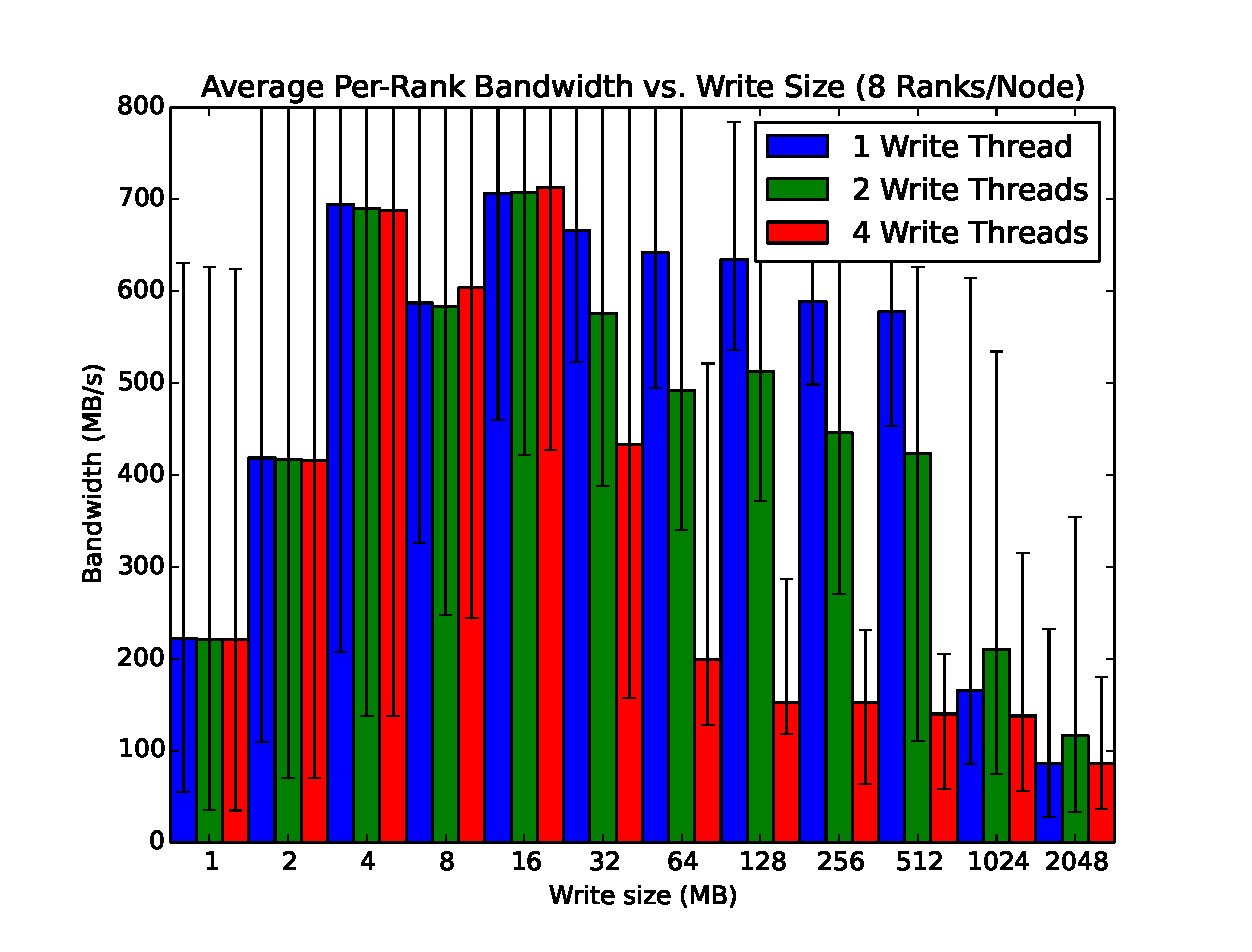
\includegraphics[width=\linewidth]{figures/figure_3.eps}
%\caption{Minimum \& maximum per-rank write bandwidth.  8 ranks per node.} 
%\label{fig:results_8_bars}
%\end{figure}

\begin{figure}
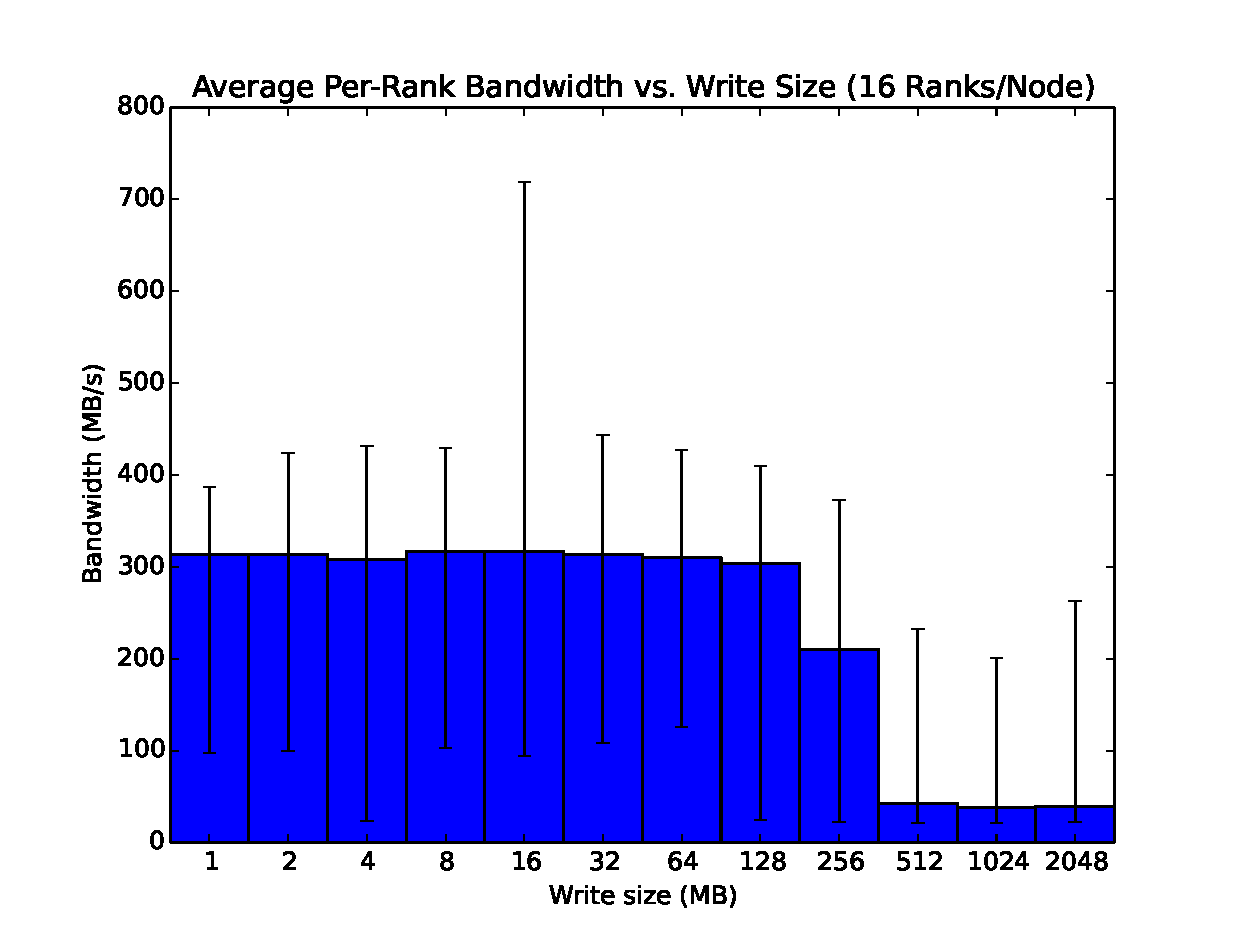
\includegraphics[width=\linewidth]{figures/figure_6.eps}
\caption{Average per-rank write bandwidth using standard \texttt{write()} calls.  16 ranks per node. No GPU memory cache.} 
\label{fig:results_base_16}
\end{figure}

\begin{figure}
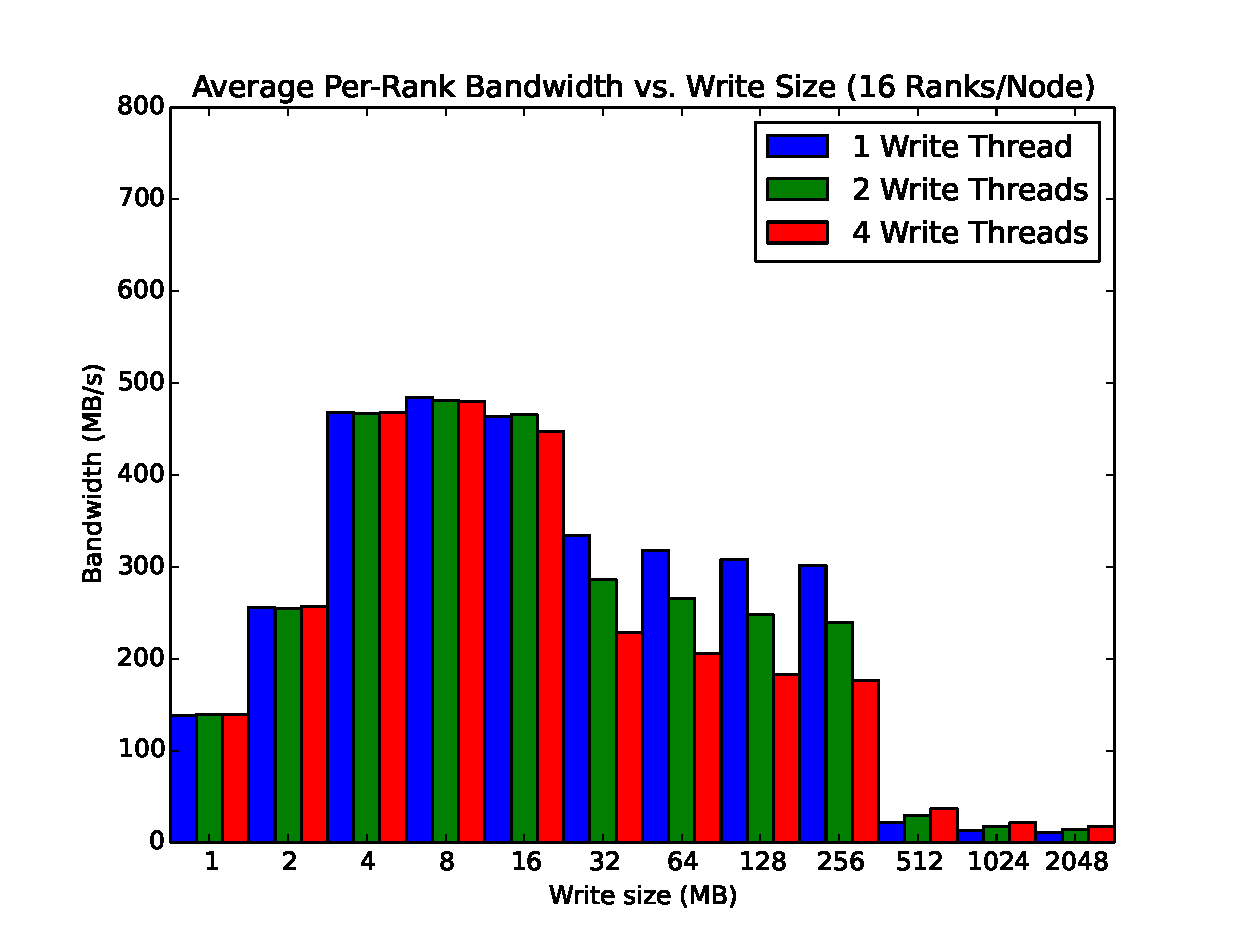
\includegraphics[width=\linewidth]{figures/figure_4.eps}
\caption{Average per-rank write bandwidth.  16 ranks per node.} 
\label{fig:results_16_nobars}
\end{figure}

%\begin{figure}
%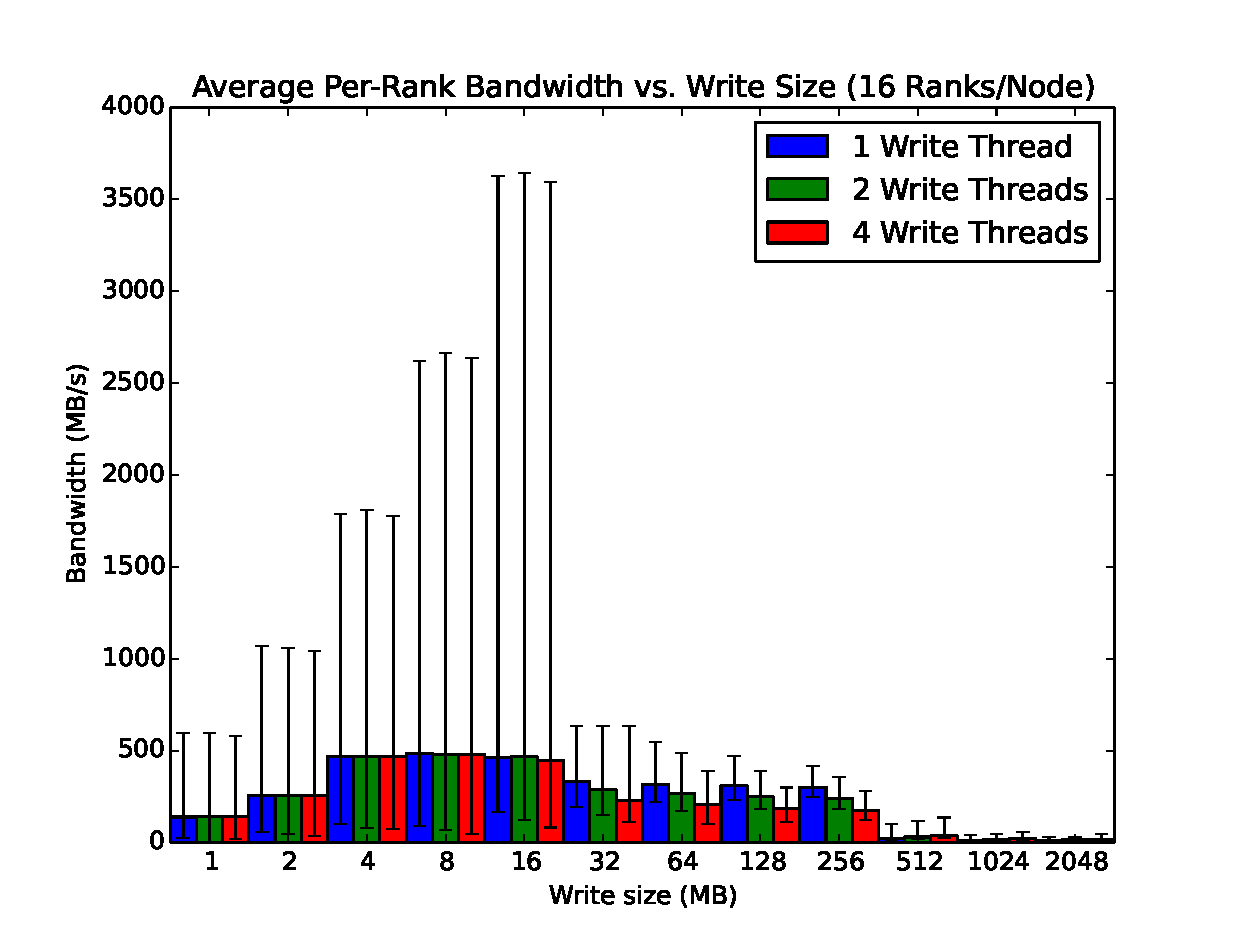
\includegraphics[width=\linewidth]{figures/figure_5.eps}
%\caption{Minimum \& maximum per-rank write bandwidth.  16 ranks per node.} 
%\label{fig:results_16_bars}
%\end{figure}

Figures \ref{fig:results_base_16} and \ref{fig:results_16_nobars} show the results for the second series of tests.  As noted above, this series used 16 ranks per node, plus the daemon's threads.  This meant, of course, that the cores were oversubscribed.  Notice that Figure \ref{fig:results_base_16} has the same basic shape as Figure \ref{fig:results_base_8}.  The only significant difference is that the reported speeds shown in Figure \ref{fig:results_base_16} are approximately half those shown in Figure \ref{fig:results_base_8}.  This is expected, since there are twice as many ranks writing. Again, the baseline test uses 128 nodes while each of the daemon with 1, 2, and 4 write threads present the mean of 64 nodes each.

Figure \ref{fig:results_16_nobars} shows that again, the per-rank bandwidth is about half that shown in Figure \ref{fig:results_8_nobars} because there are twice as many ranks.  It is also clear that the application ranks see good write performance up to the 256MB write size, which is the largest size that will entirely fit into GPU memory.  It is also clear that, as in the first test series, writes must be at least 4MB in order to get reasonable performance copying the data into GPU memory.


Looking at figure \ref{fig:results_16_nobars}, note the drop in performance between 16MB and 32MB and the slight downward trend from 32MB to 256MB.  This pattern also appears in Figure \ref{fig:results_8_nobars}, but is much more obvious in Figure 
\ref{fig:results_16_nobars}.  The authors hypothesize that this is related to the response time of the daemon.  As mentioned earlier, the daemon allocates GPU memory in blocks of up to 16MB.  Thus, if one of the ranks wants to write more than 16GB, it will need to go through more than one request/response message cycle.  However, the daemon only has a single thread to handle these messages.  When multiple ranks are sending message, they will necessarily have to wait while the daemon services any previous messages and this slows their overall performance.  This is more noticeable in Figure 
\ref{fig:results_16_nobars} because there are more ranks making requests.
In short, it appears that improving the response time of the message handling thread would be beneficial.
